%\motto{Use the template \emph{chapter.tex} to style the various elements of your chapter content.}
\chapter{Medizinische Anwendungsgebiete}
\label{trends} % Always give a unique label
% use \chaptermark{}
% to alter or adjust the chapter heading in the running head

\chapterauthor{Martin Maier, Siri Wandel}

\abstract{some abstract}

\section{Relevanz \& Problemstellung}


\section{Top 3 Anwendungsfelder (Praxis \& Theorie)}
Die potenziellen Einsatzmöglichkeiten von Quantencomputern im Gesundheitswesen sind vielfältig, wie Abbildung \ref{fig:use-cases-medicine} verdeutlicht. Sie reichen von molekularer Simulation über Krebsbehandlung bis hin zu Bildanalyseverfahren. In diesem Abschnitt liegt der Fokus auf den drei Anwendungsfeldern, die aktuell sowohl in der Forschung als auch in der industriellen Entwicklung eine herausragende Rolle spielen: Wirkstoffentwicklung , Proteinstrukturvorhersage und Personalisierte Medizin.\\

\begin{figure}[ht]
    \centering
    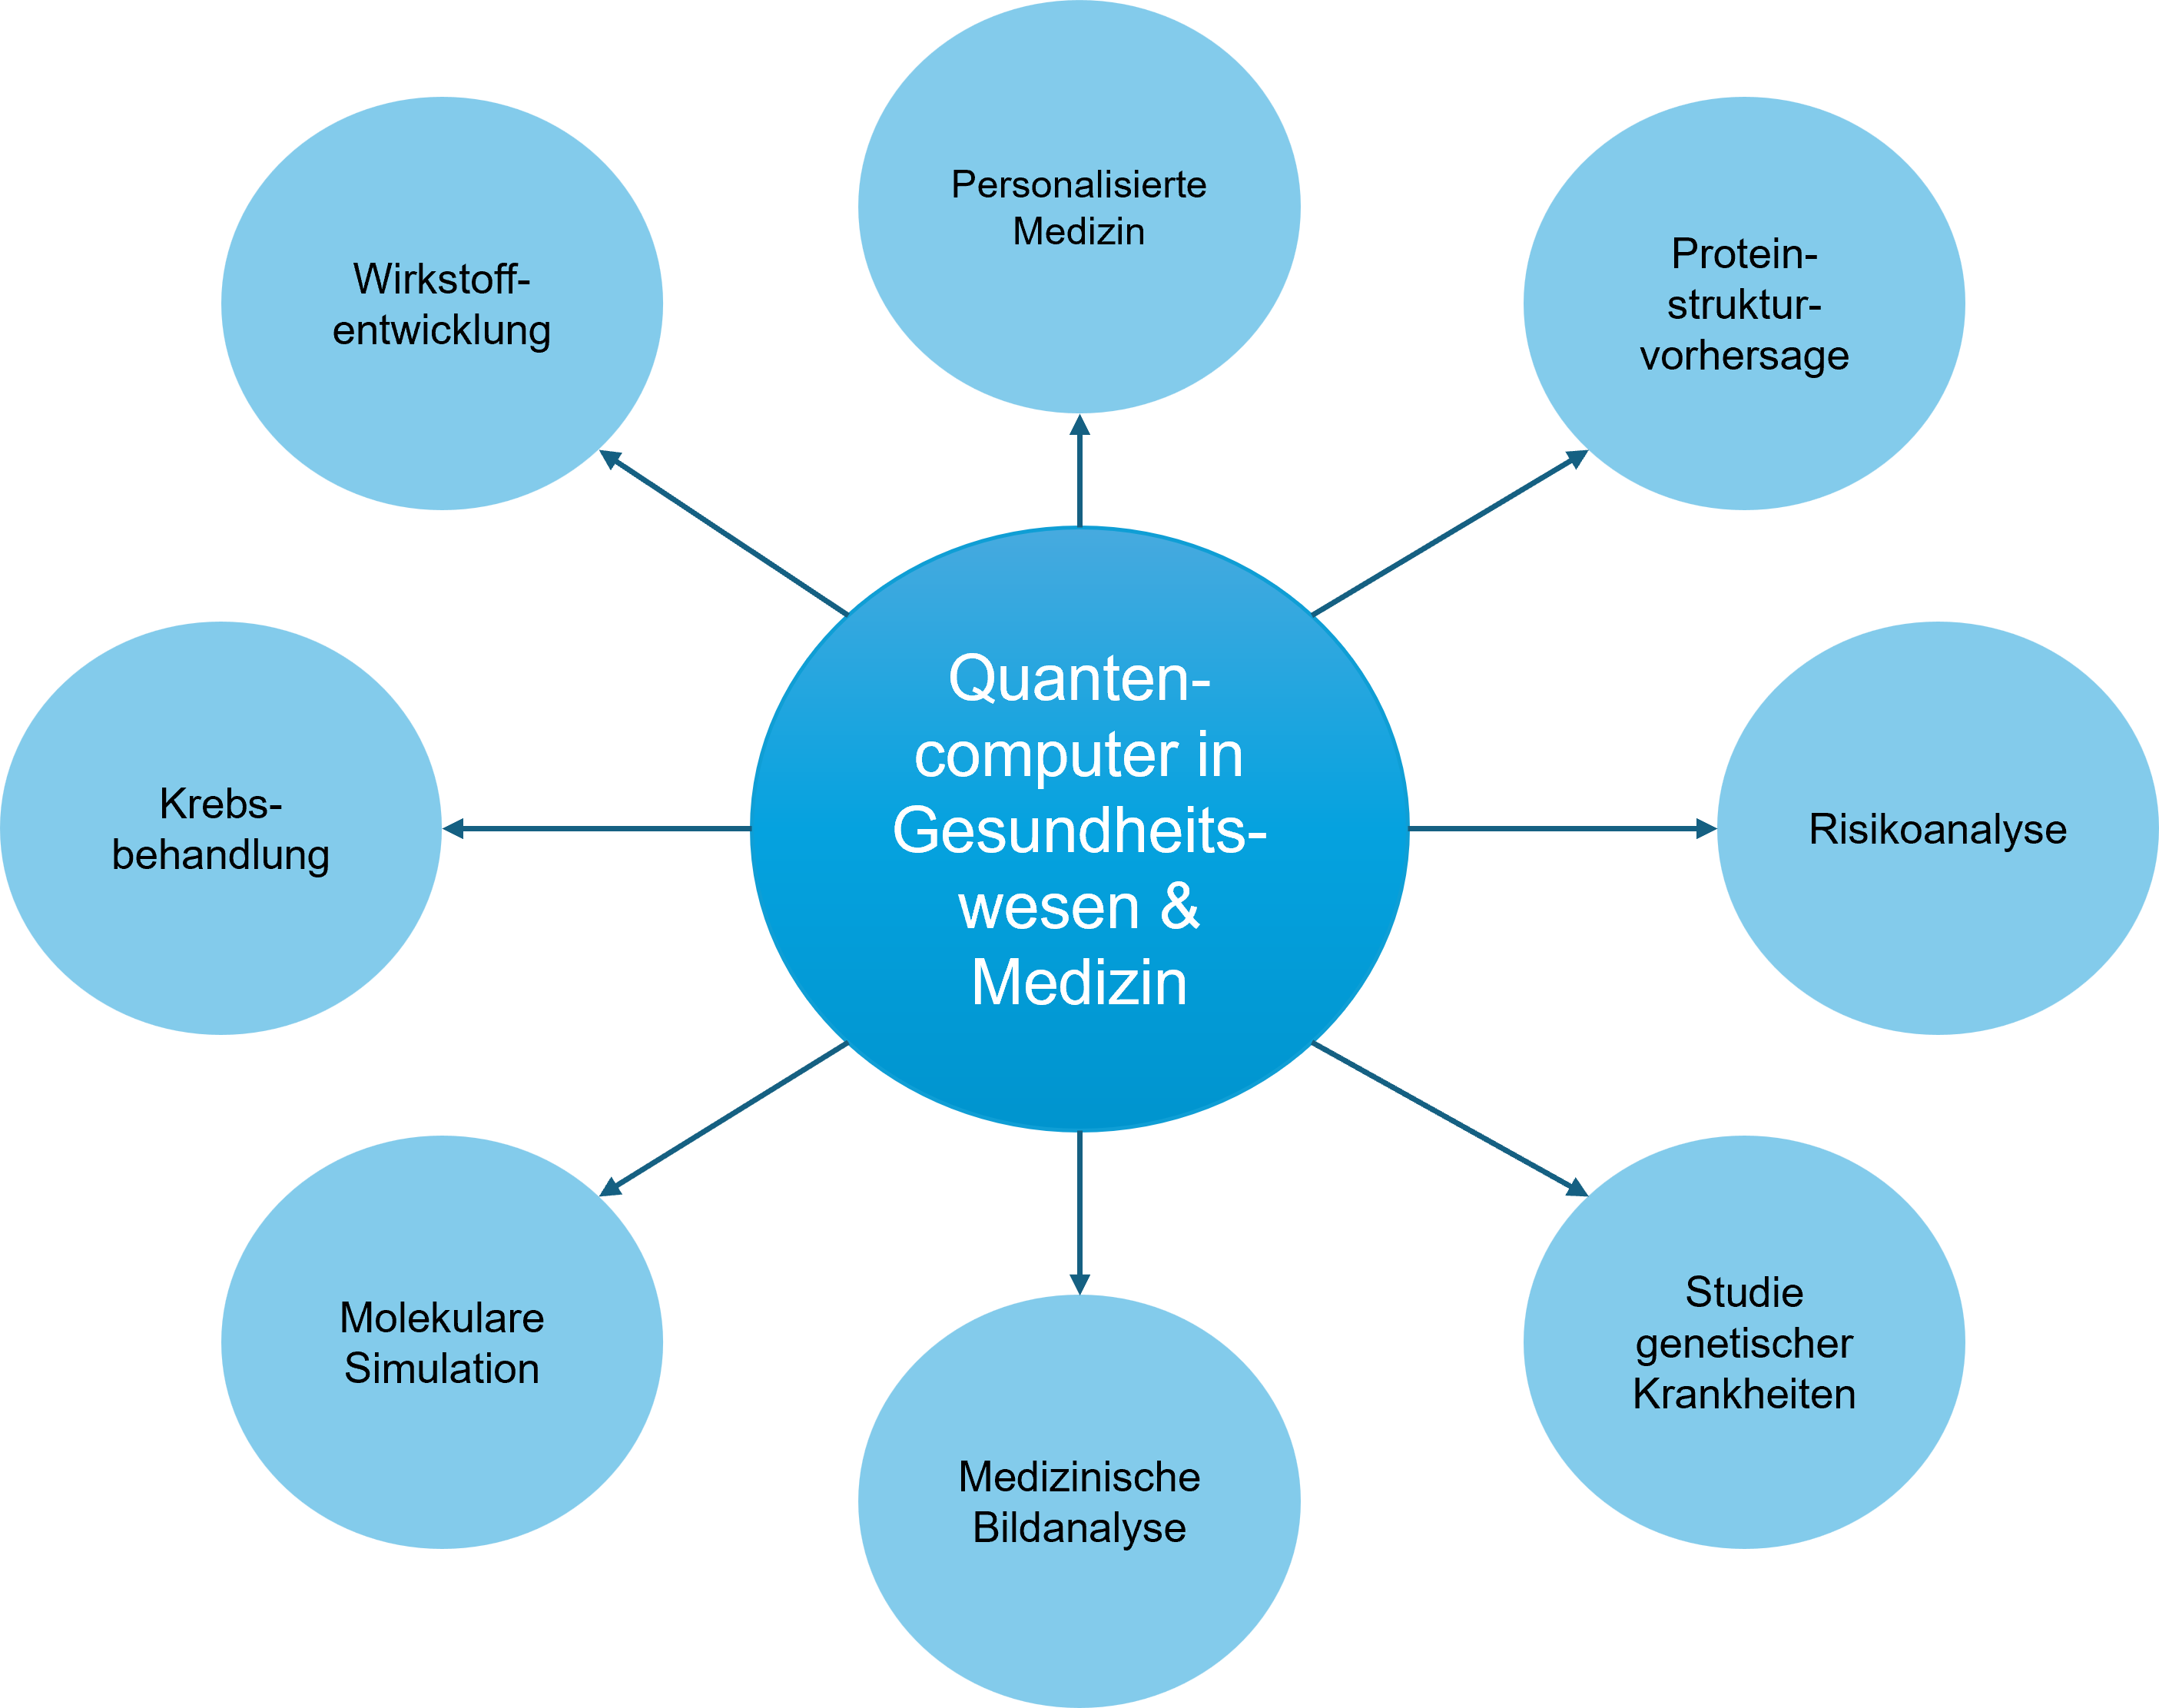
\includegraphics[width=.8\textwidth]{images/medicine/AnwendungsfelderMedizin.png}
    \caption{Übersicht möglicher Einsatzfelder von Quantencomputern in der Medizin. (Eigene Darstellung nach \cite{dhande_quantum_2023}.)}
    \label{fig:use-cases-medicine}
\end{figure}

Diese Auswahl basiert auf drei qualitativen Kriterien: Erstens adressieren diese Bereiche relevante medizinische Herausforderungen. Zweitens zeichnen sie sich durch eine besonders hohe rechnerische Komplexität aus, die den Einsatz von Quantencomputern sinnvoll erscheinen lässt. Drittens bestehen bereits erste praxisnahe Anwendungen und Pilotprojekte, die eine Brücke zwischen theoretischem Potenzial und konkreter Nutzung bilden. Die Auswahl orientiert sich somit nicht nur an theoretischem Potenzial, sondern auch an praktischer Umsetzbarkeit und gesellschaftlicher Relevanz.\\

\subsection{Wirkstoffentwicklung}
Die Entwicklung neuer Wirkstoffe ist grundlegend mit hohen Kosten verbunden. Das liegt besonders an langen Entwicklungszyklen und einer geringen Erfolgsquote. Der Einsatz von Computern, besonders im Rahmen des Computer"=Aided Drug Design (CADD), ist in der pharmazeutischen Forschung etabliert. Dies stößt jedoch bei der Modellierung komplexer molekularer Systeme an seine Grenzen (Vgl. \cite{bertl_quantum_2025}).\\

\subsubsection*{Compound Screening \& Lead"=Optimierung}
Quantencomputer versprechen, diese Prozesse durch genauere und schnellere Simulationen von Molekülen und deren Wechselwirkungen erheblich zu verbessern. Dabei konzentrieren sich aktuelle Quantencomputing"=Anwendungen in der pharmazeutischen Forschung besonders auf zwei frühe Phasen der Wirkstoffentwicklung: das \textit{Compound Screening} und die \textit{Lead"=Optimierung}. Beim Compound Screening werden sehr viele verschiedene chemische Verbindungen daraufhin untersucht, ob sie grundsätzlich an ein Zielmolekül (z.B. ein krankheitsrelevantes Protein) binden können. In der Lead"=Optimierung werden dann vielversprechende Kandidaten gezielt verbessert, um deren Wirksamkeit und Verträglichkeit zu steigern. Quantencomputer können in diesen Phasen helfen, indem sie Wechselwirkungen zwischen Molekülen genauer simulieren und energetisch günstige Strukturen besser vorhersagen (Vgl. \cite{zinner_quantum_2021}).\\

\subsubsection*{Quantenchemische Simulation}
Auf theoretischer Ebene gilt die quantenchemische Berechnung von Molekül"=Energien als eines der vielversprechendsten Anwendungsfelder des Quantencomputings. Sie ist essenziell für die Ermittlung von Bindungsaffinitäten, Reaktionspfaden und energetisch bevorzugten Konformationen, welche zentrale Größen in der computergestützten Wirkstoffentwicklung sind. Wie \cite{cao_quantum_2019} betonen: Das klassische Problem, dessen Lösung vom Quantencomputing erwartet wird, ist die Berechnung von Grundzustands- und angeregten Zustandsenergien kleiner Moleküle. Solche Berechnungen dienen als Ausgangspunkt für die Bestimmung vieler nützlicher Größen, wie etwa Reaktionspfaden, Bindungsenergien und Reaktionsgeschwindigkeiten chemischer Prozesse. (eigene Übersetzung nach \cite{cao_quantum_2019}.) Zentral ist demnach die Berechnung von Molekülenergien, da sie viele wichtige chemische Eigenschaften bestimmt.\\

\subsubsection*{Virtuelles Screening und datengetriebene Modellierung}
Beim \textit{virtuellen Screening} handelt es sich um einen frühen Schritt im Prozess der Wirkstoffentwicklung. Dabei werden mit Hilfe von Computern große Datenbanken nach Molekülen durchsucht, die an ein bestimmtes krankheitsrelevantes Ziel binden könnten. So lassen sich vielversprechende Wirkstoffkandidaten schneller finden und unnötige Labortests vermeiden. Klassische Methoden stoßen dabei aber oft an Grenzen: Die Modelle sind manchmal ungenau, liefern viele falsche Treffer und brauchen viel Rechenleistung. Neue Ansätze wie Quantum Machine Learning (siehe Kapitel \ref{alg:qml}) können hier helfen. Mit Quantencomputern lassen sich Molekülwechselwirkungen genauer simulieren und komplexe Daten effizienter verarbeiten. Techniken wie Quanten"=Neuronale Netzwerke, Quanten"=Kernel oder spezielle Quanten"=Suchalgorithmen ermöglichen ein gezielteres und schnelleres Screening. (Vgl. \cite{kumar2024})


\subsection{Proteinstrukturvorhersage}
\label{med:protein}
Die bisher etablierten Methoden zur Proteinstrukturvorhersage haben bereits beeindruckende Fortschritte erzielt. Mit experimentellen Ansätzen sowie durch KI"=basierte Modelle wie AlphaFold, RoseTTaFold und verwandte Systeme lassen sich für viele Proteine dreidimensionale Strukturen bereits mit hoher Genauigkeit vorhersagen. (Vgl. \cite{jumper2021, baek2021})\\

\subsubsection*{Grenzen klassischer Methoden}
Diese klassischen Methoden basieren meist auf Mustern aus bekannten Proteinstrukturen und liefern häufig nur ein begrenztes Verständnis der physikalischen Prozesse, die der Proteinfaltung zugrunde liegen. Das erschwert insbesondere die Vorhersage bei synthetischen oder stark abweichenden Aminosäuresequenzen. Studien zeigen, dass Modelle wie AlphaFold2 bei solchen Sequenzen außerhalb ihres Trainingsdatensatzes unzuverlässige Ergebnisse liefern können (Vgl. \cite{outeiral2022}). Physikbasierte Verfahren wie die Molekulardynamik bieten zwar grundsätzlich eine höhere Genauigkeit, sind jedoch für größere Proteine extrem rechenintensiv und in der Praxis kaum skalierbar (Vgl. \cite{doga_perspective_2024}). Diese Einschränkungen verdeutlichen den Bedarf an alternativen Modellierungsansätzen.\\

\subsubsection*{Quantenbasierte Faltungsmodelle}
Quantencomputer könnten eine vielversprechende Alternative bieten, da sie durch Quantenparallelismus potenziell viele Faltungszustände gleichzeitig analysieren können (Vgl. \cite{doga_perspective_2024}). Aktuelle Forschungsarbeiten formulieren die Proteinfaltung dabei als Optimierungsproblem und setzen auf Quantenalgorithmen sowie vereinfachte physikalische Modelle. Zwei Ansätze haben sich dabei als besonders vielversprechend erwiesen: Hybridverfahren mit VQE und quantenbasierte Gittermodelle.\\

Im Ansatz von \citeauthor{doga_perspective_2024} wurde ein hybrider Algorithmus eingesetzt, der klassische Optimierung mit einem VQE kombiniert. Ziel war die Vorhersage der Struktur eines kurzen Abschnitts mit sieben Aminosäuren aus dem Helikaseprotein des Zika"=Virus. Solche Abschnitte werden als Loops bezeichnet. Sie verbinden regelmäßige Strukturelemente wie Alpha"=Helices und Beta"=Faltblätter und sind häufig entscheidend für die Funktion eines Proteins. Die räumliche Anordnung der Atome in diesem Abschnitt, also die sogenannte Konformation, wurde anschließend mit bekannten Referenzdaten verglichen. Die mittels Quantencomputer berechnete Struktur wich deutlich weniger vom experimentell bestimmten Referenzmodell ab als die Vorhersage von AlphaFold2. Der mittlere Abstand der Atome (RMSD) betrug etwa 1,88 Å bei der Quantenmethode und 3,53 Å bei AlphaFold2. Das zeigt, dass quantenbasierte Verfahren bereits heute genauere Ergebnisse liefern können als etablierte KI"=Modelle, zumindest für kleinere, aber strukturell anspruchsvolle Proteinbereiche. (Vgl. \cite{doga_perspective_2024})\\

Ein weiterer Ansatz basiert auf Gittermodellen. \citeauthor{robert_resource-efficient_2021} verwendeten ein solches Modell zur Faltung kurzer Peptide mit IBM-Quantenhardware. Ein 10"=Aminosäure"=Peptid (Angiotensin) wurde auf 22 Qubits, ein 7-Aminosäure-Peptid auf 9 Qubits kodiert. Die Ergebnisse zeigen, dass selbst kleine Quantencomputer bereits in der Lage sind, realistische Faltungskonfigurationen effizient zu berechnen. (Vgl. \cite{robert_resource-efficient_2021})


\subsection{Personalisierte Medizin}
Die personalisierte Medizin verfolgt das Ziel, medizinische Entscheidungen stärker an den individuellen Eigenschaften eines Patienten auszurichten, etwa an genetischen Merkmalen, Krankheitsverläufen oder Therapieansprechen. Das bedeutet, dass aus komplexen, oft hochdimensionalen Daten wie Genomsequenzen, Laborwerten oder Bilddaten präzise Vorhersagen abzuleiten sind. Klassische Methoden stoßen hierbei zunehmend an ihre Grenzen, insbesondere bei kleinen Datensätzen, hoher Variabilität oder stark nichtlinearen Zusammenhängen. Auch maschinelles Lernen stoßt bei individuellen oder seltenen Fällen oft an seine Grenzen. Bei wenigen Trainingsdaten führen sie zu unsicheren Diagnosen und Therapieentscheidungen. (Vgl. \cite{gupta_systematic_2025}).\\

\subsubsection*{P5"=Medizin}
In der aktuellen Forschung wird personalisierte Medizin zunehmend als sogenanntes P5"=Modell verstanden. Dieses erweitert das bisherige P4"=Modell um eine fünfte Dimension: \textit{psychokognitiv}. Die fünf Elemente lauten: vorhersagend (predictive), vorbeugend (preventive), personalisiert, beteiligend (participatory) und psychokognitiv. Letztere betont psychologische und kognitive Faktoren wie Werte, Lebensqualität und Gesundheitskompetenz. Diese beeinflussen, wie Patienten mit Erkrankungen umgehen und wie sie auf Therapien reagieren. (Vgl. \cite{gorini_p5_2011})\\

Quantencomputing kann in diesem Kontext neue Wege eröffnen. Durch seine Fähigkeit, viele Datenmuster gleichzeitig zu analysieren, lassen sich verhaltensbezogene Einflussfaktoren stärker in personalisierte Modelle integrieren. Besonders vielversprechend ist hier der Einsatz von Quantum Machine Learning, also von Modellen, die klassische Lernverfahren mit quantenmechanischen Elementen kombinieren (Vgl. \cite{bertl_quantum_2025}.)\\

\subsubsection*{Frühe Anwendungen von Quantum Machine Learning}
Eine aktuelle Übersichtsarbeit zeigt, dass sich erste klinisch relevante QML-Anwendungen zum Beispiel in der EKG"=Analyse, Genomik oder Bildgebung bereits auf echter Quantenhardware testen lassen, wenn auch bisher in begrenztem Umfang (Vgl. \cite{gupta_systematic_2025}). Besonders Genomik und Bildgebung ermöglichen eine präzisere Diagnostik und auf individuelle genetische Profile abgestimmte Therapieansätze.\\

Ein konkretes Beispiel liefert eine Studie zur Vorhersage von Arzneimittelwirkungen bei Krebspatienten. In dieser erzielt ein hybrides QNN eine bis zu 15 Prozent höhere Genauigkeit als klassische Modelle, bei signifikant kürzerer Trainingszeit (Vgl. \cite{sagingalieva_hybrid_2023}).\\

\begin{table}[ht]
\centering
\renewcommand{\arraystretch}{1.3}
\resizebox{\textwidth}{!}{
\begin{tabular}{|p{2.3cm}|p{4.5cm}|p{2.5cm}|p{4.5cm}|}
\hline
\textbf{Anwendungsfeld} & \textbf{Rechnerische Herausforderung} & \textbf{Quantenansatz / Algorithmus} & \textbf{Warum QC relevant?} \\
\hline
Drug Discovery & Molekül-Energieberechnung, Bindungsaffinitäten & VQE, QPE & Klassische Methoden zu ungenau oder zu langsam \\
\hline
Proteinstruktur & Kombinatorische Explosion möglicher Faltungen & QAOA, Hybridalgorithmen & QC kann Zustände simultan analysieren \\
\hline
Personalisierte Medizin & Mustererkennung in hochdimensionalen Daten & QML, QNN & Klassische Modelle überfordert bei komplexer Nichtlinearität \\
\hline
\end{tabular}
}
\caption{Anwendungsfelder des Quantencomputings in der Medizin und Pharmazie}
\label{tab:qc_medizin}
\end{table}



\section{Top Technologien \& Algorithmen}

\subsection{Technologische Frameworks}

\subsubsection*{Wirkstoffentwicklung}
Die praktische Umsetzung der Quantenalgorithmen für medizinische Anwendungen erfordert leistungsfähige Software"=Stacks, die Quanten-Hardware und klassische Algorithmen verbinden. Für die Wirkstoffentwicklung werden vor allem Frameworks genutzt, die komplexe \textit{Molekül"=Hamilton"=Operatoren} bearbeiten und Verfahren wie VQE oder QPE effizient implementieren. Dabei handelt es sich um mathematische Ausdrücke, die alle relevanten physikalischen Eigenschaften eines Moleküls quantenmechanisch beschreiben. Der Hamilton-Operator bildet somit die Grundlage für die Simulation von Molekülzuständen, da er die Energieverteilung eines Systems vollständig bestimmt (Vgl. \cite{mcardle}). So bietet IBM Qiskit mit dem Qiskit Nature"=Modul spezialisierte Werkzeuge zur Darstellung chemischer Systeme und zum Lösen von Grundzustandsproblemen in Molekülen. (Vgl. \cite{noauthor_qiskit_2022})\\

Microsofts Q\# Quantum Development Kit (QDK) enthält ebenfalls eine Chemie-Bibliothek mit qubitisierten Fermionen-Operatoren sowie Implementierungen von Hamilton-Simulatoren (Trotterisierung, Qubitierung). (Vgl. \cite{msazure}) \\

Zudem erlaubt Amazon Braket als Cloud-Service den Zugriff auf unterschiedliche Quantenprozessoren (z.B. Rigetti"=Supraleiter, IonQ-Ionenfallen) und Simulationsengines über ein einheitliches SDK. (Vgl. \cite{aws})\\

Dieser flexible Ansatz wird beispielsweise im AWS-Toolkit QCEDD genutzt, das eingebaute Beispiele für Aufgaben wie molekulares Docking und Faltungsprobleme in der Wirkstoffforschung enthält. (Vgl. \cite{amazonscience})\\ %evtl. git repo zitieren

%besonders beim virtuellen screening relevant 

\subsubsection*{Proteinstrukturvorhersage}
Die Vorhersage von Proteinstrukturen ist ein hochdimensionales Optimierungsproblem. Klassischerweise modelliert man Proteine auf Gitternetzen, um die Konformationsräume lösbar zu machen. Wie bereits in Kapitel \ref{med:protein} dargelegt, sind Quantenoptimierungsalgorithmen wie QAOA dafür gut geeignet. (Vgl. \cite{boulebnane})\\

Zur praktischen Umsetzung von Algorithmen wie QAOA in der Proteinstrukturvorhersage wird geeignete Software benötigt, die die Komplexität quantenmechanischer Optimierung handhabbar macht. Ein bekanntes Framework in diesem Bereich ist \textit{PennyLane}. Es ist eine plattformunabhängige Open"=Source"=Bibliothek für Quantencomputing und Quantum Machine Learning, die für wissenschaftliche Anwendungen entwickelt wurde. Durch PennyLane können Quantenalgorithmen mit klassischen Lernverfahren kombiniert werden. Das ist besonders bei der Proteinstrukturvorhersage von Vorteil, da hier sowohl quantenbasierte Optimierung, als auch klassische Auswertungsverfahren erforderlich sind. (Vgl. \cite{PennyLane})\\

Das Start"=up Menten AI nutzt PennyLane für die Entwicklung neuer proteinbasierter Wirkstoffe. Ziel ist es, Quantencomputing und klassische Verfahren so zu kombinieren, dass neue Wirkstoffkandidaten schneller und gezielter gefunden werden können. Dabei setzt Menten AI auf PennyLane, um Quantenalgorithmen effizient einzubinden und bioaktive Peptide für neue Therapien zu entwickeln. Das heißt, sie nutzen die Software, um schneller passende Wirkstoffe zu finden, die gut an bestimmte Krankheitsziele andocken können. (Vgl. \cite{xanadu2022})\\



\subsubsection*{Personalisierte Medizin}
In der personalisierten Medizin stehen große, hochdimensionale Datensätze (Genomik, Bildgebung, EKG, klinische Parameter) im Mittelpunkt. Hier kommen Frameworks zum Einsatz, die Quantenmodelle in klassische Machine"=Learning"=Pipelines einbetten. Ein Beispiel ist die Kombination aus \textit{Cirq} und \textit{TensorFlow Quantum}. Damit lassen sich Quantenalgorithmen direkt in klassische Lernmodelle integrieren. So entstehen hybride neuronale Netze, die klassische und quantenbasierte Rechenschritte verbinden. Das hilft dabei, komplexe medizinische Daten genauer auszuwerten und Muster zu erkennen, die für individuelle Behandlungsentscheidungen wichtig sind. (Vgl. \cite{tensorflowQuantum2020})

\section{Wichtige Unternehmen \& Akteure}


\section{Top 3 Zukunftsprojekte \& Forschungsinitiativen}


\section{Bewertung anhand der Kriterien}


\section{Teilfazit}


\printbibliography
